\subsection{Relaciones Estructurales}

Las relaciones estructurales representan la coherencia "estática" dentro de una arquitectura.  El concepto de composición (el lado "de" de la relación) es siempre un elemento; el concepto de composición (el lado "de" de la relación) puede en algunos casos ser también otra relación.

\begin{table}[h!]
	\subsubsection{Elementos}
	\begin{center}
		\begin{tabular}{| l | l | r |}
			\hline
			Concepto & Descripción & Representación \\ \hline
			
			Agregación 
			&
			\begin{tabular}[l]{@{}l@{}}
				Indica que un elemento consiste en \\
				uno u otros conceptos más.
			\end{tabular}
			& \includegraphics[width=0.4\linewidth]{imgs/relaciones/agregacion}
			\\\hline
			
			Composición
			& 
			\begin{tabular}[l]{@{}l@{}}
				Indica que un elemento consiste en \\
				uno u otros conceptos más.
			\end{tabular}
			& \includegraphics[width=0.4\linewidth]{imgs/relaciones/composicion}
			\\\hline
			
			Asignación
			& 
			\begin{tabular}[l]{@{}l@{}}
				Expresa la asignación de \\
				responsabilidad, la ejecución \\
				de la conducta, o la ejecución.
			\end{tabular}
			& 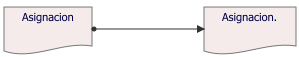
\includegraphics[width=0.4\linewidth]{imgs/relaciones/asignacion}
			\\\hline
			
			Realización
			& 
			\begin{tabular}[l]{@{}l@{}}
				Indica que una entidad desempeña \\
				un papel fundamental en la creación,\\
				el logro, el sustento o el \\
				funcionamiento de una entidad más \\
				abstracta.
			\end{tabular}
			& 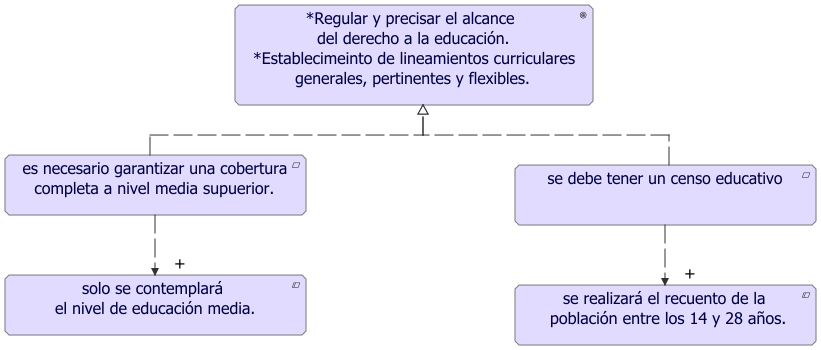
\includegraphics[width=0.4\linewidth]{imgs/relaciones/realizacion}
			\\\hline
			
		\end{tabular}
		\caption{Relaciones estructurales}
		\label{tab:estructurales}
	\end{center}
\end{table}